%告知 CTeX 这个文件是用 UTF-8 编码
% !Mode:: "TeX:UTF-8"

%使用 pdflatex
%!TEX program = pdflatex


\documentclass[12pt,a4paper]{article}
%正文字体大小为12pt, 页面规格是A4, 使用article文档格式
\usepackage[utf8]{inputenc}
%作用是inputenc用来识别输入编码
\usepackage[left=2.2cm,right=2.2cm,top=3cm,bottom=2.5cm]{geometry}
%latex设置页面边距,页面大小,页边距
\usepackage{mathtools}
%数学公式扩展宏包,提供了公式编号定制和更多的符号、矩阵等
\usepackage{booktabs}  
%booktabs宏包画三线表,线条精细可变
\usepackage{graphicx} 
%支持插图
\usepackage{listings}
%提供了排版关键字高亮的代码环境 lslisting 以及对版式的自定义。
%类似宏包有minted

\lstset{%使用\lstset{}进行代码环境的设置
backgroundcolor=\color{cyan!10},%% 选择代码背景,必须加上\ usepackage {color}或\ usepackage {xcolor}.
basicstyle=\ttfamily, % 设置代码字号.
numbers=left,% 给代码添加行号,可取值none, left, right.
numberstyle=\scriptsize %小六号 \scriptsize
% numberstyle=\tiny\color{mygray}, % 行号的字号和颜色
}

\usepackage{fancyhdr}
%修改页眉页脚格式,令页眉页脚可以左对齐、居中、右对齐

\usepackage{tikz}%以 TikZ 为基础提供排版样式丰富的彩色盒子的功能
\usepackage[europeanresistors,americaninductors]{circuitikz}
%欧式电阻,美式电感

\usepackage{indentfirst} %令章节标题后的第一段首行缩进
\usepackage[wby]{callouts}

\lstdefinestyle{mystyle}{
    backgroundcolor=\color{white},  %背景颜色 
    commentstyle=\color{codegreen}, %注释风格
    keywordstyle=\color{magenta},   %关键字风格 红紫色
    numberstyle=\tiny\color{codegray},
    stringstyle=\color{codepurple},
    basicstyle=\footnotesize\ttfamily,breaklines=true,
    %设置代码的大小  选择一种等宽(“打字机”)字体族  对过长的代码自动换行  
    breakatwhitespace=false, %空格中断
    xleftmargin=20pt, %x左边框
    xrightmargin=20pt,%x右边框       
    breaklines=true,  %代码过长则换行               
    captionpos=b,     % 设置标题位置.               
    keepspaces=true,  % 保留空格    有助于保持代码的缩进 possibly needs columns=flexible           
    numbers=left,     % 给代码添加行号,可取值none, left, right.                   
    numbersep=5pt,    % 设置行号与代码之间的间隔              
    showspaces=false, % 显示每个地方添加特定下划线的空格; 覆盖了'showtringspaces'               
    showstringspaces=false, % 仅在字符串中允许空格
    showtabs=false,   % 在字符串中显示添加特定下划线的制表符               
    tabsize=2,        % 将默认tab设置为2个空格  
    framextopmargin=50pt,%代码区定框
    frame=bottomline,   %代码区底部
    basicstyle=\footnotesize\ttfamily,  % 设置代码字号
    language=Octave     % 使用的语言
}
\usepackage{ulem}%提供排版可断行下划线的命令 \uline 以及其它装饰文字的命令
\lstset{style=mystyle} %代码环境设置  自定义版式,将mystyle中版式导入
\linespread{1.5}       %行距1.5倍 
\title{\textbf{\texttt{Exercises}}}
\author{Automation Class 1904}
\pagestyle{fancy}   %使用fancy风格
\fancyhf{} % 清空当前设置
\rhead{Exercise} %页眉右边
\rfoot{fireowl}       %页脚右边
\lhead{Electric Circuits} % 页眉左边
\cfoot{\thepage}    %页脚中间 页码
\thispagestyle{plain}
% empty
% 无页眉页脚
% plain
% 无页眉,页脚为居中页码
% headings
% 页眉为章节标题,无页脚
% myheadings
% 页眉内容可自定义,无页脚
\date{(Due date: 2020/12/25)}%自定义日期\date{(Due date: 2020/10/5)} \today显示电脑上的日期-英文版


\begin{document}


%section
\begin{enumerate}
	\item
	\begin{quote}
		The relay shown in Fig. P7.103 connects the 30 V
		dc generator to the dc bus as long as the relay current
		is greater than 0.4 A. If the relay current
		drops to 0.4 A or less, the spring-loaded relay
		immediately connects the dc bus to the 30 V
		standby battery. The resistance of the relay winding
		is $ 60\Omega $. The inductance of the relay winding is
		to be determined.\\
		\\
		a) Assume the prime motor driving the 30 V dc
		generator abruptly slows down, causing the
		generated voltage to drop suddenly to 21 V.
		What value of L will assure that the standby
		battery will be connected to the dc bus in
		0.5 seconds?\\
		\\
		b) Using the value of L determined in (a), state
		how long it will take the relay to operate if the
		generated voltage suddenly drops to zero.

		
		\begin{center}
			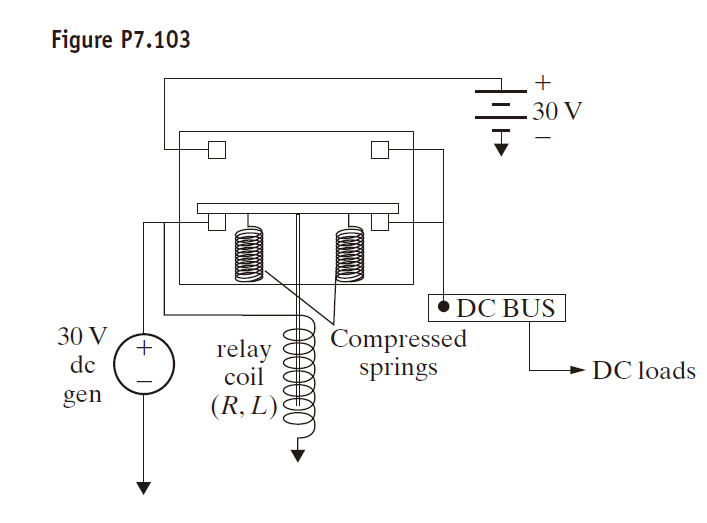
\includegraphics[width=0.4\textheight]{s1_1.png}
		\end{center}
	\end{quote}	

	\clearpage

		

	
    \begin{quote}
    	Ans:\\
    	Convert to circuit diagram:
    	\begin{center}
    		\begin{circuitikz}[american]
    			\draw
    			(1,3) node[cute spdt down] (Sw) {}
    			%(Sw.in) %node[left] {}
    			(Sw.out 2) %node[left] {}
    			(Sw.out 1); %node[right] {};
    			
    			\draw(0,0) to [V, l = 30V, invert] (0,3) to(Sw.in);
    			\draw (Sw.out 1) to [V, l=30V, invert] (5,3.43) to [short,-*] (5,3);
    			\draw (Sw.out 2) to  (5,2.57)to (5,3);
    			
    			\draw (5, 3) to (6,3) to [L, l= L] (6,1.5)
    			to[R, l= 60$\Omega$] (6,0) to(0,0);
    			
    			\node at  (1.23,3.58) {a};
    			\node at  (1.23,2.28) {b};
    			
    		\end{circuitikz}
    	\end{center}
    	a).From the question that we can known :
    	\begin{center}
    		$I_s = \frac{21}{60}A$ \qquad $I_0 = \frac{30}{60}A$ \qquad $\tau  = \frac{L}{R} = \frac{L}{60}$
    	\end{center}
    	Then we can calculate i(t):
    	\begin{center}
    		$i(t) = I_s + (I_0 - I_s)e^{-\frac{t}{\tau}}$\\
    		$i(t) = 0.35 + 0.15e^{-\frac{60t}{L}}$
    	\end{center}
    	If we want assure that the standby battery will be connected to the dc bus in 0.5 seconds.\\We need i(0.5) = 0.4A:
    	\begin{center}
    		$i(t) = 0.35 + 0.15e^{-\frac{30}{L}} = 0.4$
    	\end{center}
    	Since we can calculate L:
    	\begin{center}
    		$L = \frac{30}{ln3} = 27.31H$
    	\end{center}
    	b).Because of the generate voltage suddenly drops to zero (V: 30V $\rightarrow$ 0V)\\
    	Thus:
    	\begin{center}
    		$i(t) = 0 + (\frac{30}{60} - 0)e^{-\frac{60t}{L}} = 0.5e^{-\frac{60t}{27.31}}$ \qquad(L = 27.31H)
    	\end{center}
    	When the relay to operate that i$>$0.4, so at i = 0.4 this time the relay will release:
    	\begin{center}
    		$i =  0.5e^{-\frac{60t}{27.31}} = 0.4$
    	\end{center}
    	Thus:
    	\begin{center}
    		$t = \frac{27.31ln1.25}{60} \cong 0.1s $
    	\end{center}
    	
    	
    \end{quote}
   			
    

\end{enumerate}
\end{document}